\documentclass[11pt,landscape]{article}
\usepackage{geometry} % Pour passer au format A4
\geometry{hmargin=1cm, vmargin=0.6cm} % 

% Page et encodage
\usepackage[T1]{fontenc} % Use 8-bit encoding that has 256 glyphs
\usepackage[english,french]{babel} % Français et anglais
\usepackage[utf8]{inputenc} 

\usepackage{lmodern}
\setlength\parindent{0pt}

% Graphiques
\usepackage{graphicx,float,grffile}

% Maths et divers
\usepackage{amsmath,amsfonts,amssymb,amsthm,verbatim}
\usepackage{multicol,enumitem,url,eurosym,gensymb}

% Sections
\usepackage{sectsty} % Allows customizing section commands
\allsectionsfont{\centering \normalfont\scshape}

% Tête et pied de page

\usepackage{fancyhdr} 
\pagestyle{fancyplain} 

\fancyhead{} % No page header
\fancyfoot{}

\renewcommand{\headrulewidth}{0pt} % Remove header underlines
\renewcommand{\footrulewidth}{0pt} % Remove footer underlines

\newcommand{\horrule}[1]{\rule{\linewidth}{#1}} % Create horizontal rule command with 1 argument of height

%----------------------------------------------------------------------------------------
%   Début du document
%----------------------------------------------------------------------------------------

\begin{document}


\setlength{\columnseprule}{1pt}

\horrule{2px}
\section*{DM - Modélisation du monde}
\horrule{2px}
\vspace{-1cm}

\subsection*{Les domaines de l'informatique}

Lancer la vidéo sur Youtube : \url{https://youtu.be/SzJ46YA_RaA}

Après avoir choisi un domaine informatique parmi tous ceux qui sont encadrés. 

\textbf{Marquer le titre en gros, mettre une traduction, expliquer en quelques phrases et mettre quelques photos ou dessins si cela est possible.}

    \begin{figure}[H]
        \centering
        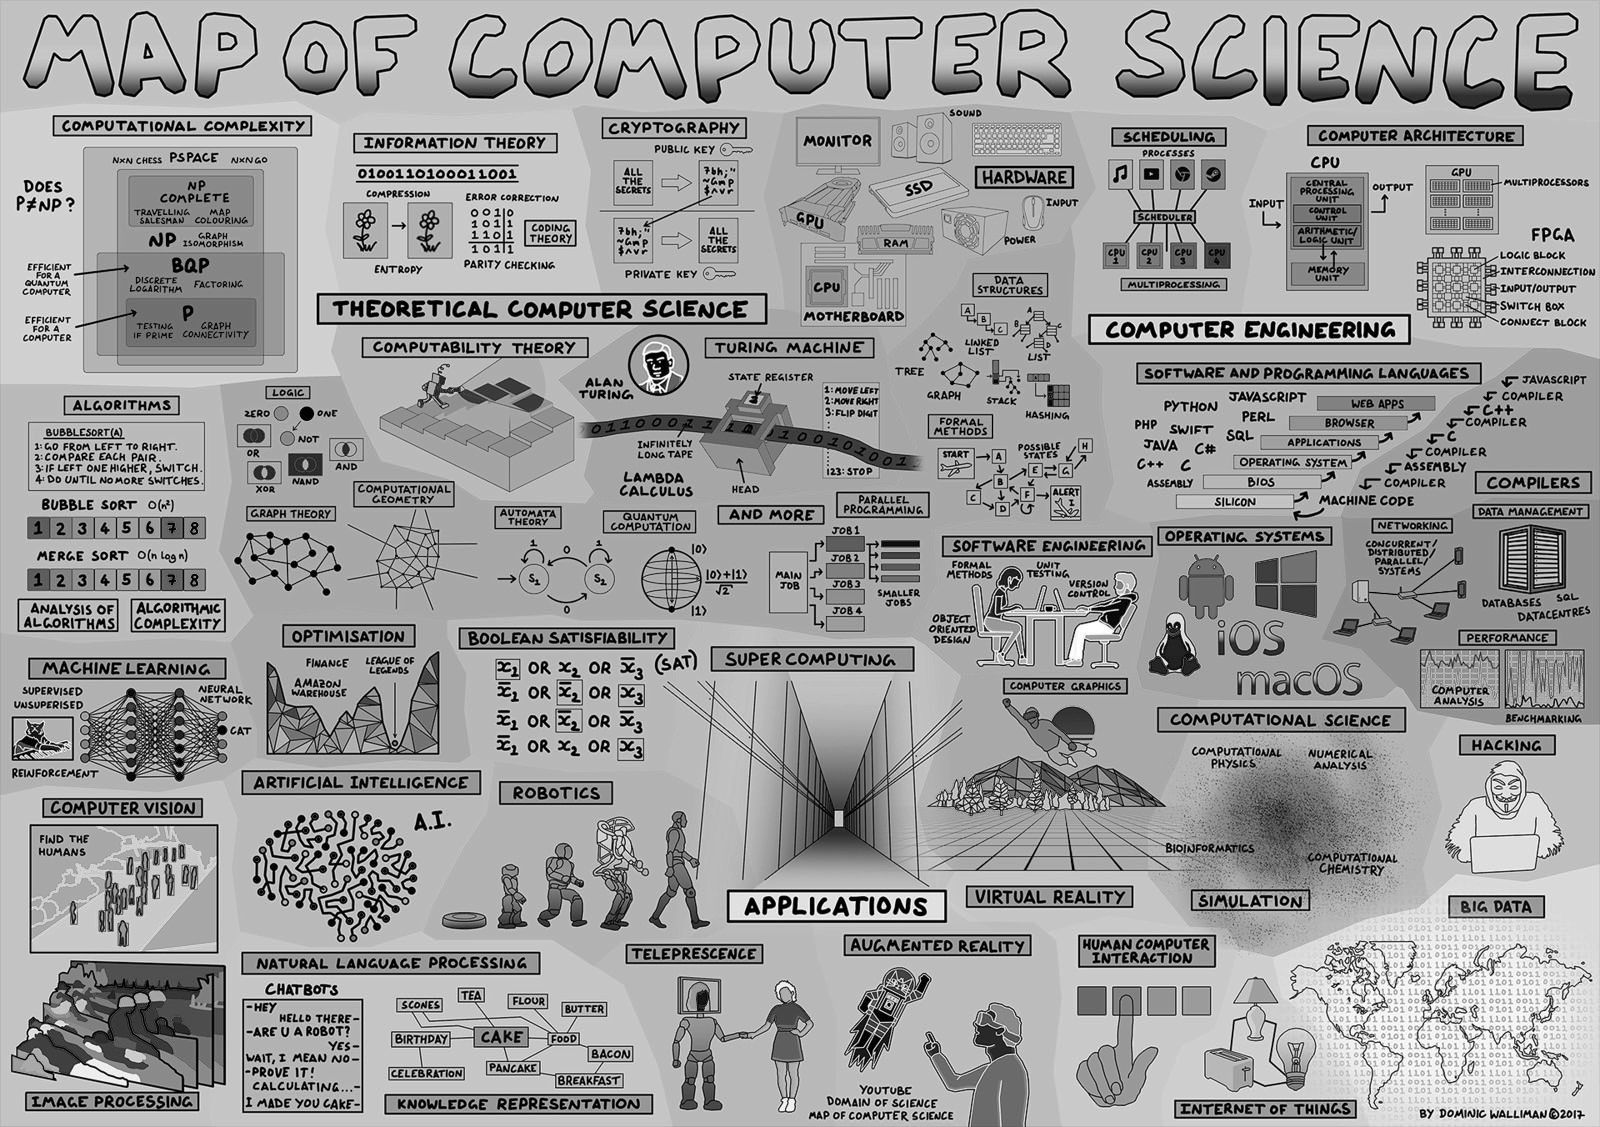
\includegraphics[width=0.8\linewidth]{4x5-calcul-litteral-1/sources/compsci-2.png}
  \end{figure}

\end{document}
